In order to test the created agent the data that where splitted for training are used and to present the result a Confusion Matrix was created. In that way it can be seen how many of the true lables the model was able to predict after the training and the results are the following :
\begin{figure}[H]
    \centering
    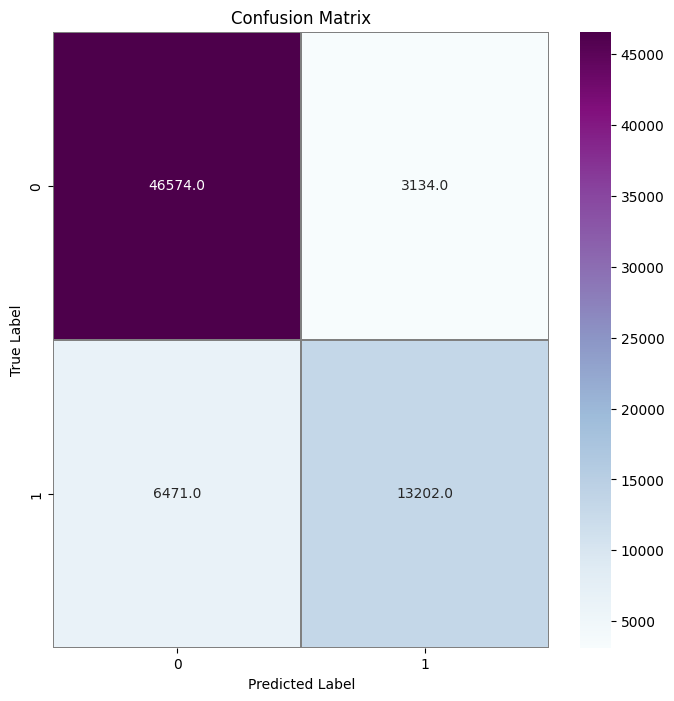
\includegraphics[width=0.7\textwidth]{Images/confusion.png}
    \caption{Data Split}
    \label{fig:example}
\end{figure}
In that way it is observed that works pretty well in general terms since the accuracy of the prediction was at the 84,9\%, a percentage near to the one that was achieved in training. However, even thought in the negative cases the model predicts succesfully the 93.7\% of the cases as negative, in the positive cases it performs significantly lower at 67.1\%, but that is probably due to the unbalanced dataset, that as we can see in \autoref{fig:Figure1} it has much more negative cases than positive (198,738 IDC negative and 78,786 IDC positive).